\documentclass[conf]{new-aiaa}
%\documentclass[journal]{new-aiaa} for journal papers
\usepackage[utf8]{inputenc}
\usepackage{float}
\usepackage{multirow} % for multi-row cells
\usepackage{array} % for customized column formatting
\usepackage[ruled,vlined]{algorithm2e}
\usepackage{graphicx}
\usepackage{amsmath}
\usepackage[version=4]{mhchem}
\usepackage{siunitx}
\usepackage{longtable,tabularx}
\setlength\LTleft{0pt} 

\title{AE 598-RL HW1 Report}

\author{Gokul Puthumanaillam (gokulp2)}
\affil{Department of Aerospace Engineering, University of Illinois Urbana-Champaign}

\begin{document}

\maketitle


\section{Problem Description}
\subsection{Grid World}
The setting for this environment is a grid layout, comprising of 5 columns and 5 rows. The entire grid comprises of 25 different states, each representing a unique location. There are four feasible actions that can be taken at each state: right, up, left, and down. The environment's transition model is defined, and all algorithms have access to it. The objective of the algorithms is to learn how to navigate through the environment and find a path that maximizes the episode reward. This task will require the algorithms to identify the optimal sequence of actions to take in order to achieve the highest reward possible.

\subsection{Inverted Pendulum}
This environment comprises a simple pendulum with a discretized state and action space. The transition model for this environment is not explicitly available. The state of the pendulum is determined by the angle $\theta$ displacement from the vertical axis. The maximum allowed angular velocity of the pendulum is fixed (exceeding which, a large negative reward is incurred). The objective of the algorithm is to maintain the pendulum's state within a specific goal range, which represents an upright position, and rewards a score of +1. Any state outside the goal range earns a score of 0. Therefore, the algorithms will be trained to maintain the pendulum inverted for as many time-steps as possible during an episode. This will require the algorithm to balance the pendulum by selecting the appropriate actions at each time step.

\section{Preliminaries}
This report documents the generated graphs for the following algorithms in the Grid World and the Discrete Pendulum (in a tabular setting):
\begin{enumerate}
    \item Value Iteration: Grid World
    \item Policy Iteration: Grid World
    \item SARSA: Grid World and Discrete Pendulum
    \item QLearning: Grid World and Discrete Pendulum
\end{enumerate}

\begin{algorithm}[H]
\SetAlgoLined
\KwIn{MDP $M = (\mathcal{S}, \mathcal{A}, P, R, \gamma)$}
\KwOut{Optimal value function $V^*$}
\textbf{Initialization:} $V_0(s) \gets 0, \forall s \in \mathcal{S}$\;
\For{$i=1$ \KwTo $\infty$}{
    \For{$s \in \mathcal{S}$}{
        $V_{i}(s) \gets \max_{a \in \mathcal{A}} \left( R(s,a) + \gamma \sum_{s' \in \mathcal{S}} P(s'|s,a) V_{i-1}(s') \right)$\;
    }
    \If{$\|V_i - V_{i-1}\|_\infty < \epsilon$}{
        \textbf{Break}\;
    }
}
\Return{$V_i$}
\caption{Value Iteration}
\end{algorithm}

\begin{algorithm}[H]
\SetAlgoLined
\KwIn{MDP $M = (\mathcal{S}, \mathcal{A}, P, R, \gamma)$}
\KwOut{Optimal policy $\pi^*$}
\textbf{Initialization:} $\pi_0(s) \gets \text{arbitrary}, \forall s \in \mathcal{S}$\;
\For{$i=0$ \KwTo $\infty$}{
    \textbf{Policy Evaluation:}\;
    \quad $V^{\pi_i}(s) \gets \sum_{a \in \mathcal{A}} \pi_i(a|s) \left( R(s,a) + \gamma \sum_{s' \in \mathcal{S}} P(s'|s,a) V^{\pi_i}(s') \right), \forall s \in \mathcal{S}$\;
    \textbf{Policy Improvement:}\;
    \quad $\pi_{i+1}(s) \gets \arg\max_{a \in \mathcal{A}} \left( R(s,a) + \gamma \sum_{s' \in \mathcal{S}} P(s'|s,a) V^{\pi_i}(s') \right), \forall s \in \mathcal{S}$\;
    \If{$\pi_{i+1} = \pi_i$}{
        \textbf{Break}\;
    }
}
\Return{$\pi_i$}
\caption{Policy Iteration}
\end{algorithm}


\begin{algorithm}[H]
\SetAlgoLined
\KwIn{Environment with state-action pairs $Q$, initial state $s$, exploration rate $\epsilon$, learning rate $\alpha$, discount factor $\gamma$}
\KwOut{Learned action-value function $Q$}
\textbf{Initialization:} $Q(s,a) \gets \text{arbitrary}, \forall a$\;
\textbf{Repeat for each episode:}\;
\quad Initialize $s$\;
\quad Choose $a$ using $\epsilon$-greedy policy based on $Q$\;
\quad \textbf{Repeat for each step:}\;
\quad \quad Take action $a$, observe $r$ and $s'$\;
\quad \quad Choose $a'$ using $\epsilon$-greedy policy based on $Q$\;
\quad \quad $Q(s,a) \gets Q(s,a) + \alpha (r + \gamma Q(s',a') - Q(s,a))$\;
\quad \quad $s \gets s'$, $a \gets a'$\;
\quad Until $s$ is terminal\;
\Return{$Q$}
\caption{SARSA}
\end{algorithm}



\begin{algorithm}[H]
\SetAlgoLined
\KwIn{Environment with state-action pairs $Q$, initial state $s$, exploration rate $\epsilon$, learning rate $\alpha$, discount factor $\gamma$}
\KwOut{Learned action-value function $Q$}
\textbf{Initialization:} $Q(s,a) \gets \text{arbitrary}, \forall a$\;
\textbf{Repeat for each episode:}\;
\quad Initialize $s$\;
\quad \textbf{Repeat for each step:}\;
\quad \quad Choose $a$ using $\epsilon$-greedy policy based on $Q$\;
\quad \quad Take action $a$, observe $r$ and $s'$\;
\quad \quad $Q(s,a) \gets Q(s,a) + \alpha (r + \gamma \max_{a'} Q(s',a') - Q(s,a))$\;
\quad \quad $s \gets s'$\;
\quad Until $s$ is terminal\;
\Return{$Q$}
\caption{Q-learning}
\end{algorithm}

\section{Hyperparameters:}

\subsection{Grid World}
\subsubsection{Value Iteration and Policy Iteration}
\begin{enumerate}
    \item Max Number of episodes: 5000
    \item $\gamma$: 0.95
    \item $\theta$=1e-6
\end{enumerate}


\subsubsection{SARSA and QLearning}
\begin{enumerate}
    \item Max Number of episodes: 5000
    \item $\gamma$: 0.95
    \item $\theta$: 1e-6
    \item $\epsilon$: 0.1
\end{enumerate}


\subsection{Discrete Pendulum}

\subsubsection{SARSA and QLearning}
\begin{enumerate}
    \item Max Number of episodes: 700
    \item $\gamma$: 0.95
    \item $\theta$: 1e-6
    \item $\epsilon$: 0.1
\end{enumerate}




\section{Plots}
\subsection{Grid World}
\begin{figure}[H]
\centering
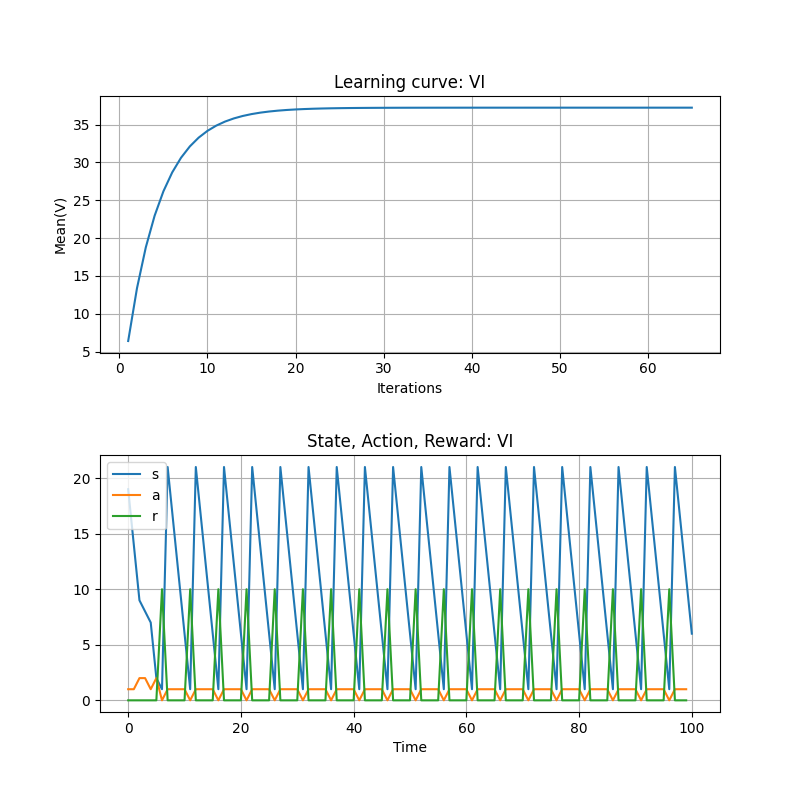
\includegraphics[width=30pc]{figs/gw/learning_and_trajectory_vi.png}
\caption{Plots showing the learning curve for Value Iteration and the State, Action, Rewards}
\label{fig_env1}
\end{figure}

\begin{figure}[H]
\centering
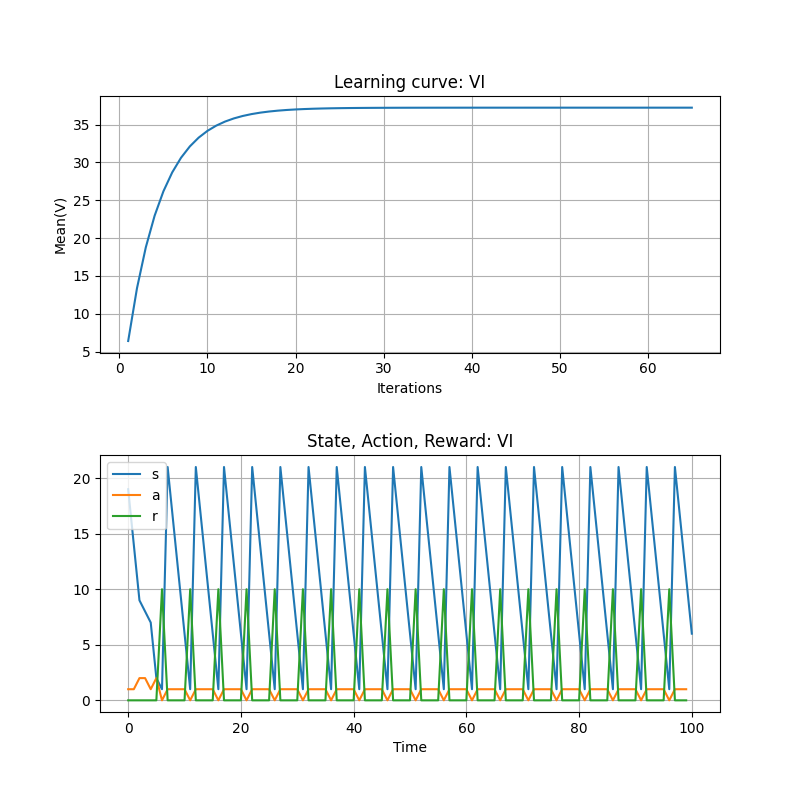
\includegraphics[width=30pc]{figs/gw/learning_and_trajectory_vi.png}
\caption{Plots showing the learning curve for Policy Iteration and the State, Action, Rewards}
\label{fig_env1}
\end{figure}

\begin{figure}[H]
\centering
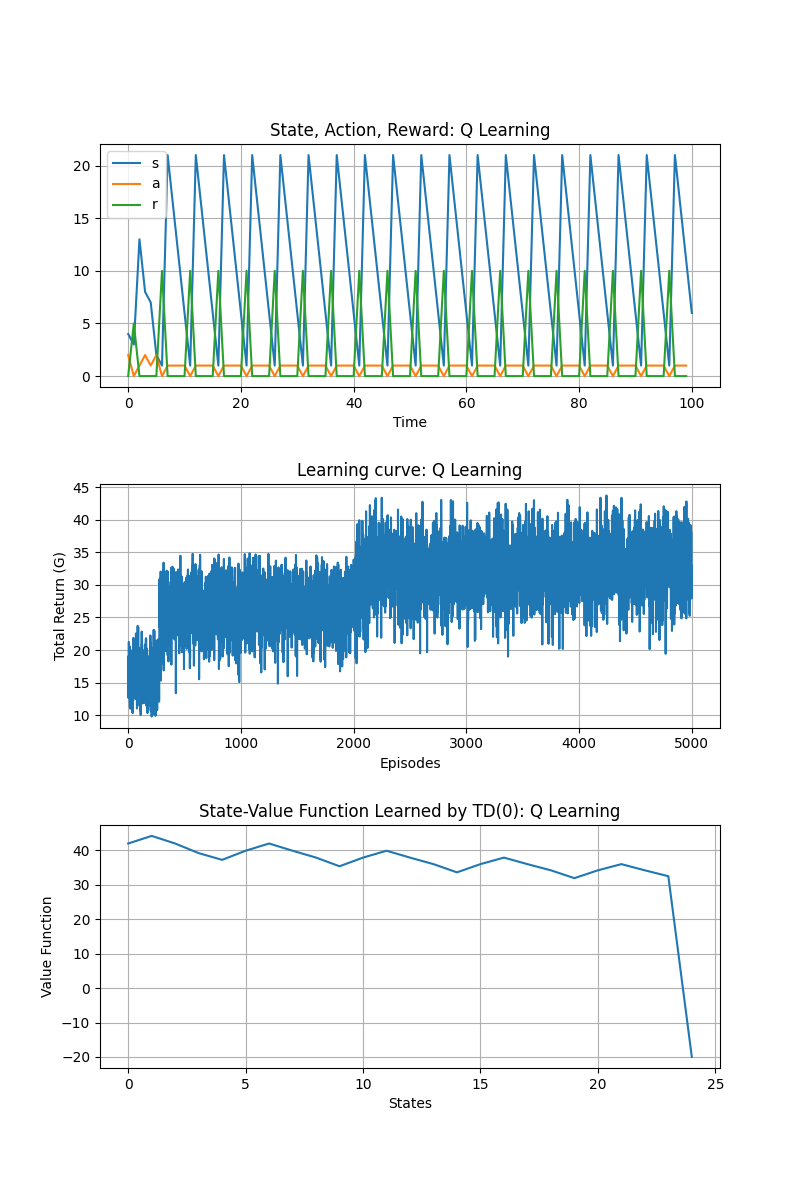
\includegraphics[width=30pc]{figs/gw/qlearning_plots.png}
\caption{Plots for QLearning: (a)State, Action, Reward (b) Learning Curve (c) State Value Function Estimation using TD(0)}
\label{fig_env1}
\end{figure}



\begin{figure}[H]
\centering
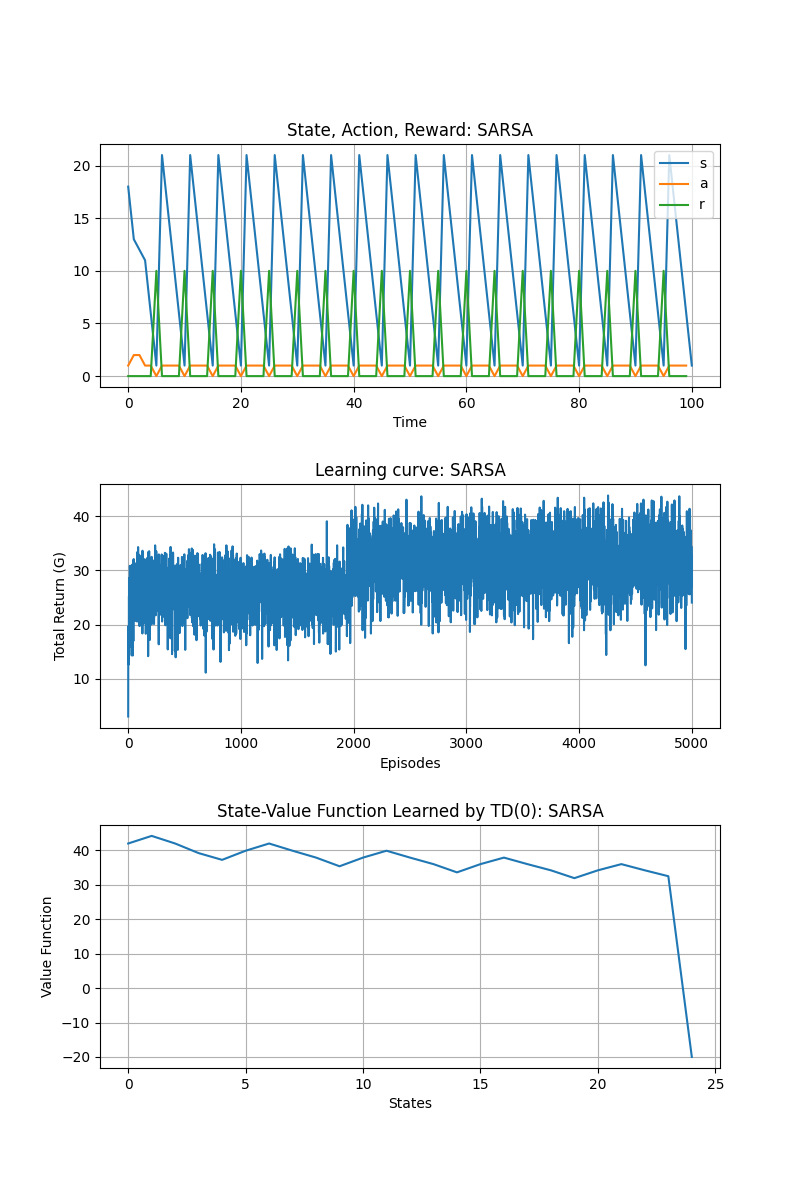
\includegraphics[width=30pc]{figs/gw/sarsa_plots.png}
\caption{Plots for SARSA: (a)State, Action, Reward (b) Learning Curve (c) State Value Function Estimation using TD(0)}
\label{fig_env1}
\end{figure}




\begin{figure}[H]
\centering
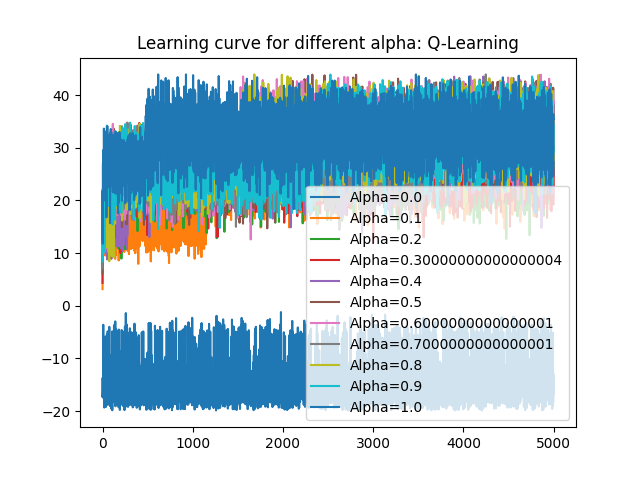
\includegraphics[width=30pc]{figs/gw/alpha_sweep_qlearning.png}
\caption{Learning Curve for different Alpha: QLearning}
\label{fig_env1}
\end{figure}

\begin{figure}[H]
\centering
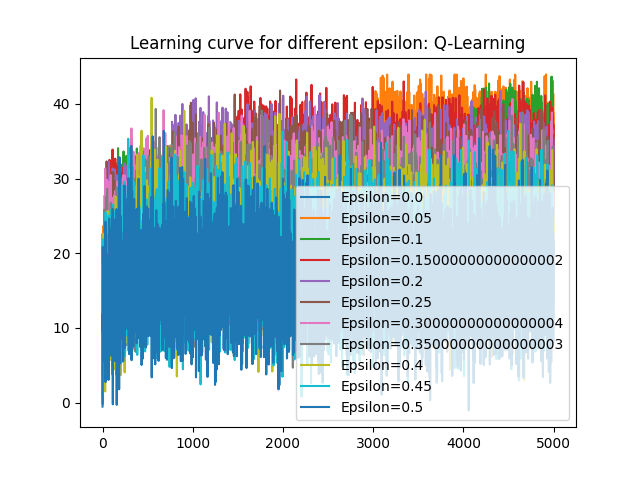
\includegraphics[width=30pc]{figs/gw/epsilon_sweep_qlearning.png}
\caption{Learning Curve for different Epsilon: QLearning}
\label{fig_env1}
\end{figure}




\begin{figure}[H]
\centering
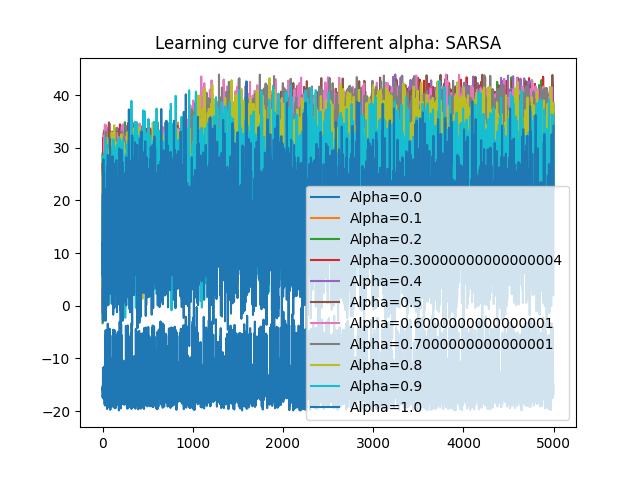
\includegraphics[width=30pc]{figs/gw/alpha_sweep_SARSA.png}
\caption{Learning Curve for different Alpha: SARSA}
\label{fig_env1}
\end{figure}

\begin{figure}[H]
\centering
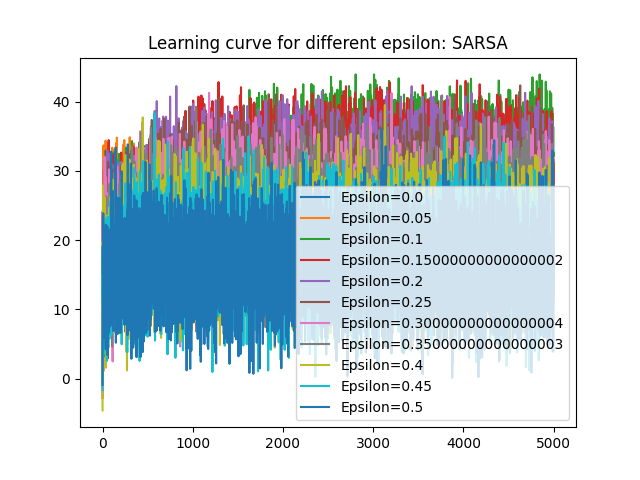
\includegraphics[width=30pc]{figs/gw/epsilon_sweep_SARSA.png}
\caption{Learning Curve for different Epsilon: SARSA}
\label{fig_env1}
\end{figure}





\newpage
\subsection{Discrete Pendulum}


\begin{figure}[H]
\centering
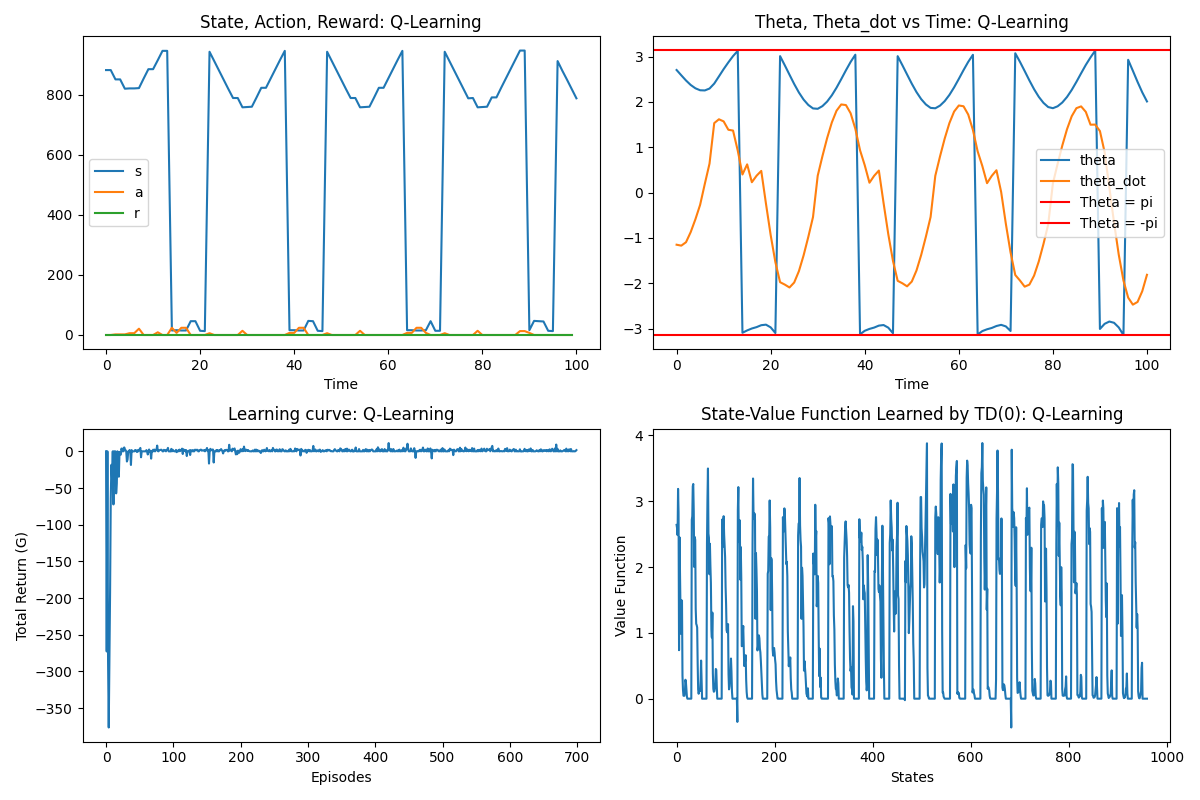
\includegraphics[width=30pc]{figs/pen/subplots_qlearning.png}
\caption{Plots for QLearning: (a)State, Action, Reward (b) Theta, Theta dot vs time(c) Learning Curve (d) State Value Function Estimation using TD(0)}
\label{fig_env1}
\end{figure}


\begin{figure}[H]
\centering
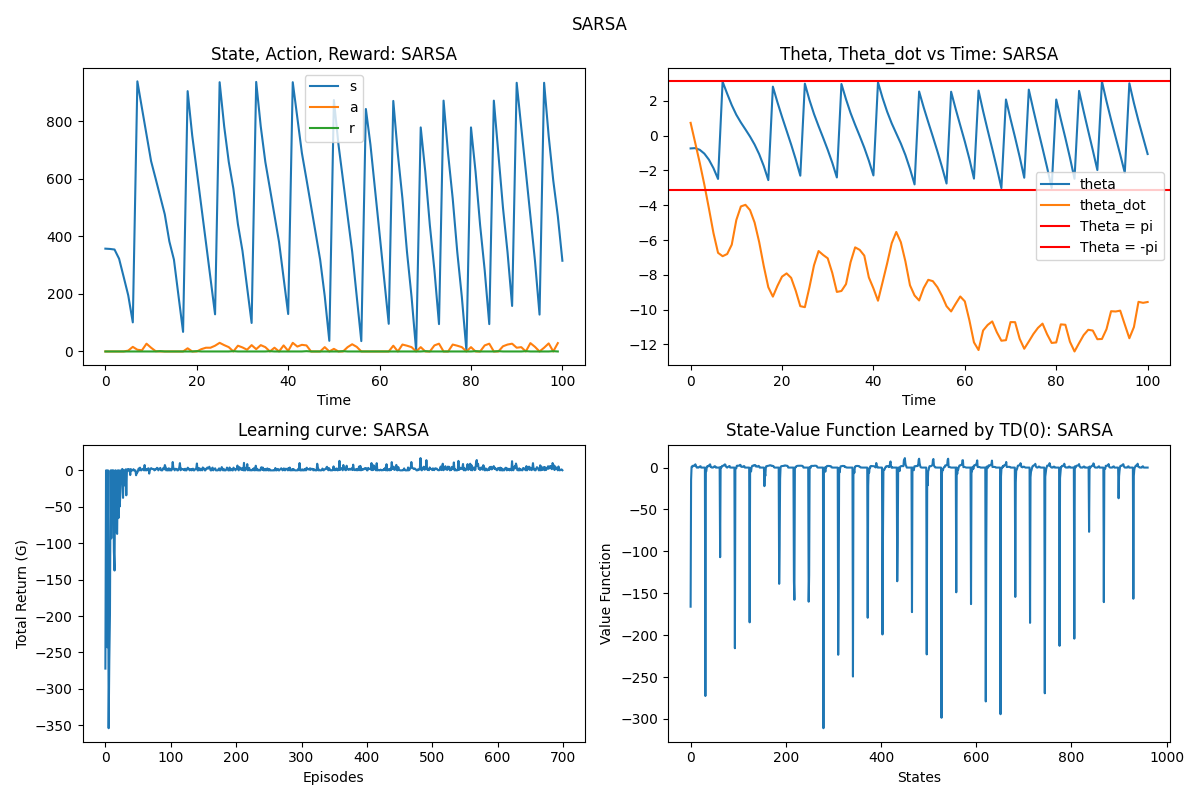
\includegraphics[width=30pc]{figs/pen/sarsa_plots.png}
\caption{Plots for SARSA: (a)State, Action, Reward (b) Theta, Theta dot vs time(c) Learning Curve (d) State Value Function Estimation using TD(0)}
\label{fig_env1}
\end{figure}




\begin{figure}[H]
\centering
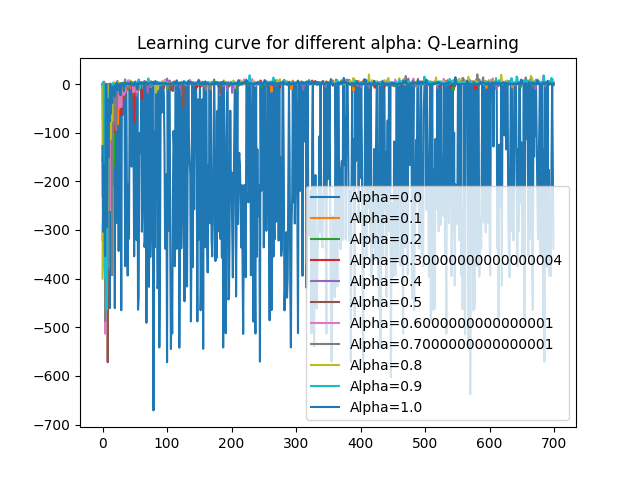
\includegraphics[width=30pc]{figs/pen/alpha_sweep_qlearning.png}
\caption{Learning Curve for different Alpha: QLearning}
\label{fig_env1}
\end{figure}


\begin{figure}[H]
\centering
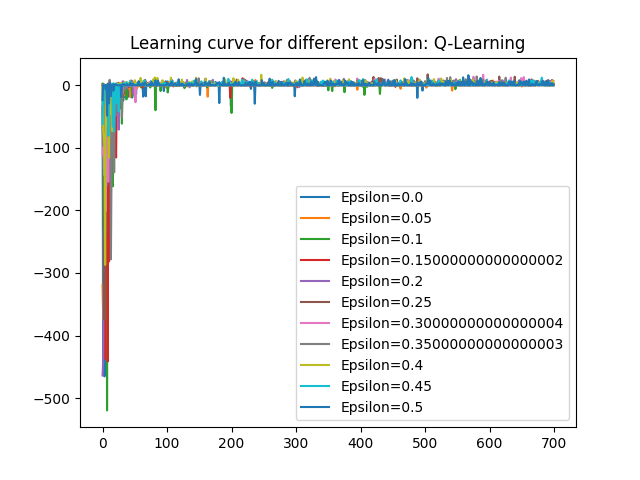
\includegraphics[width=30pc]{figs/pen/epsilon_sweep_qlearning.png}
\caption{Learning Curve for different Epsilon: QLearning}
\label{fig_env1}
\end{figure}


\begin{figure}[H]
\centering
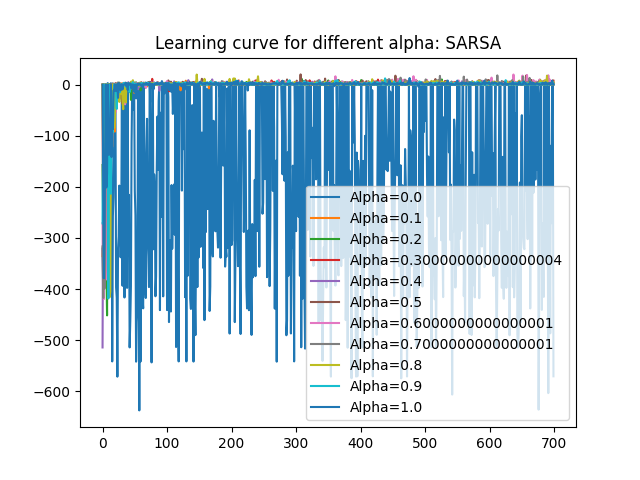
\includegraphics[width=30pc]{figs/pen/alpha_sweep_SARSA.png}
\caption{Learning Curve for different Alpha: SARSA}
\label{fig_env1}
\end{figure}


\begin{figure}[H]
\centering
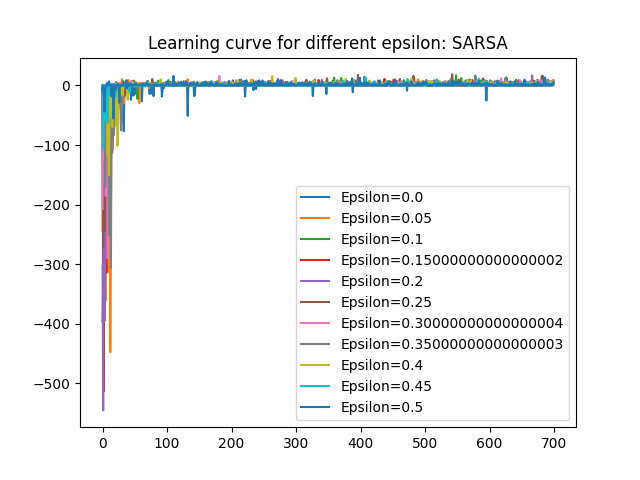
\includegraphics[width=30pc]{figs/pen/epsilon_sweep_SARSA.png}
\caption{Learning Curve for different Epsilon: SARSA}
\label{fig_env1}
\end{figure}


\end{document}
